\documentclass{beamer}


\mode<presentation>
{
  \usetheme{CambridgeUS}
	\usecolortheme{beaver}
  % or ...

  \setbeamercovered{transparent}
  % or whatever (possibly just delete it)
}


\usepackage{xeCJK}
\usepackage[english]{babel}
\usepackage[utf8]{inputenc}
\usepackage{times}
\usepackage[T1]{fontenc}
\usepackage{hyperref}
\usepackage{pifont}
\usepackage{bibentry}
\usepackage{verbatim}
\newcommand{\cmark}{\ding{51}}%
\newcommand{\xmark}{\ding{55}}%
\setCJKmainfont{WenQuanYi Micro Hei}


\title[开源软件基础] 
{开源软件基础}
\subtitle{概念与历史}

\author[Zhilei Ren] 
{Zhilei Ren}

\institute[OSCAR Team] % (optional, but mostly needed)
{
\\
\includegraphics[width=0.2\textwidth]{logo.jpg}\\
OSCAR Team, School of Software, 
Dalian University of Technology
}


\subject{Scientific Writing}



\pgfdeclareimage[height=0.5cm]{university-logo}{logo.jpg}
\logo{\pgfuseimage{university-logo}}



% Delete this, if you do not want the table of contents to pop up at
% the beginning of each subsection:
\AtBeginSubsection[]
{
  \begin{frame}<beamer>{Outline}
    \tableofcontents[currentsection,currentsubsection]
  \end{frame}
}


% If you wish to uncover everything in a step-wise fashion, uncomment
% the following command: 

%\beamerdefaultoverlayspecification{<+->}

\setbeamertemplate{section in toc}[circle]
\setbeamertemplate{items}[circle]
\setbeamertemplate{caption}[numbered]
\setbeamertemplate{bibliography item}{\insertbiblabel}
\setbeamertemplate{bibliography entry title}{}
\setbeamertemplate{bibliography entry journal}{}

\begin{document}

\begin{frame}
  \titlepage
\end{frame}

%\begin{frame}{Outline}
%  \tableofcontents[currentsection,currentsubsection, 
%    hideothersubsections, 
%    sectionstyle=show,
%]
%\end{frame}

\AtBeginSection[]
{
 \begin{frame}<beamer>
 \frametitle{Outline}
 \tableofcontents[currentsection]
 \end{frame}
}
\section{关于我}
\begin{frame}
\frametitle{关于我}
\begin{block}{任志磊}
	\begin{itemize}
		\item 副教授
		\item 2003年进入软件学院学习
		\item \url{http://oscar-lab.org/people/~zren}
		\item \href{mailto:zren@dlut.edu.cn}{\texttt{zren@dlut.edu.cn}}
		\item 研究兴趣: 

			\begin{itemize}
				\item 进化计算
				\item 数据挖掘
				\item 软件工程应用
			\end{itemize}

%		\item OSCAR stands for ``Optimizing Software by Computation from ARtificial intelligence''
%			\pause
%		\item or ``Operating System will Crash whenever my Algorithm Runs''
		\item \scriptsize{\url{https://bitbucket.org/rezilla/open-lecture-notes.git}}
	\end{itemize}
\end{block}
\end{frame}
\begin{frame}
\frametitle{所在团队}
\begin{block}{OSCAR}
	\begin{itemize}
		\item 江贺教授团队
		\item \url{http://oscar-lab.org}
		\item ``\textbf{O}ptimizing \textbf{S}oftware by \textbf{C}omputation from \textbf{AR}tificial intelligence''
			\pause
		\item or ``\textbf{O}perating \textbf{S}ystem will \textbf{C}rash whenever my \textbf{A}lgorithm \textbf{R}uns''
	\end{itemize}
\end{block}
\end{frame}

\section{定义}
\begin{frame}
  \frametitle{开源软件的定义}
	\begin{block}{定义}
		开放源代码的定义由Bruce Perens（Debian的创始人之一）定义如下：
		\scriptsize
		\begin{itemize}
			\item 自由再散布（Free Distribution）：允许获得源代码的人可自由再将此源代码散布。
			\item 源代码（Source Code）：程序的可执行文件在散布时，必需以随附完整源代码或是可让人方便的事后获取源代码。
			\item 派生著作（Derived Works）：让人可依此源代码修改后，在依照同一许可协议的情形下再散布。
			\item 原创作者程序源代码的完整性（Integrity of The Author’s Source Code）：意即修改后的版本，需以不同的版本号码以与原始的代码做分别，保障原始的代码完整性。
			\item 不得对任何人或团体有差别待遇（No Discrimination Against Persons or Groups）：开放源代码软件不得因性别、团体、国家、族群等设置限制，但若是因为法律规定的情形则为例外（如：美国政府限制高加密软件的出口）。
		\end{itemize}
	\end{block}
\end{frame}
\begin{frame}
  \frametitle{开源软件的定义（续）}
	\begin{block}{定义}
		\scriptsize
		\begin{itemize}
			\item 对程序在任何领域内的利用不得有差别待遇（No Discrimination Against Fields of Endeavor）：意即不得限制商业使用。
			\item 散布许可协议（Distribution of License）：若软件再散布，必需以同一条款散布之。
			\item 许可协议不得专属于特定产品（License Must Not Be Specific to a Product）：若多个程序组合成一套软件，则当某一开放源代码的程序单独散布时，也必需要匹配开放源代码的条件。
			\item 许可协议不得限制其他软件（License Must Not Restrict Other Software）：当某一开放源代码软件与其他非开放源代码软件一起散布时（例如放在同一光盘），不得限制其他软件的授权条件也要遵照开放源代码的授权。
			\item 许可协议必须技术中立（License Must Be Technology-Neutral）：意即许可协议不得限制为电子格式才有效，若是纸本的许可协议也应视为有效。
		\end{itemize}
	\end{block}
\end{frame}
\begin{frame}
  \frametitle{开源软件的历史}
	\begin{block}{}
		\scriptsize
1997年，Eric Raymond出版其著作《大教堂和市集》，探讨黑客社区与自由软件原则。1998年初，该论文受到极大的关注，为促成网景通信公司将其受欢迎的互联网套装软件Netscape释放成为自由软件的因素之一。这些代码即为今日大家熟悉的Mozilla Firefox与Thunderbird。

网景的行动激起Raymond及其伙伴深入研究如何将自由软件基金会的自由软件概念及优点带入商业软件产业。他们查觉基金会的社会活动不如网景等公司的行动来得吸引人，因而试图重新包装自由软件运动，以强调分享与协作软件源代码的潜在商机。他们选用的新名称为“开放源代码”（open source），很快地布鲁斯·佩伦斯、出版家提姆·奥莱理、林纳斯·托瓦兹及其他人支持新名称。开放源代码促进会于1998年2月创建，以推动使用新名称，并宣扬开放源代码的原则。
		
	\end{block}
	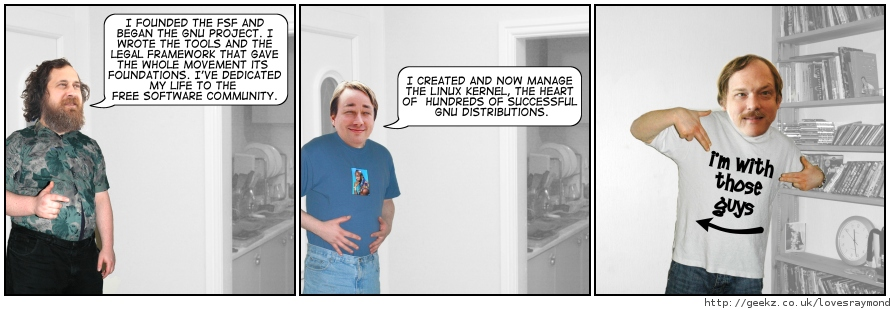
\includegraphics[width=.7\textwidth]{eric.jpg}
	
\end{frame}

\begin{frame}
  \frametitle{向前追溯}
	\begin{block}{UNIX vs. GNU vs. Linux}
		\scriptsize
		\begin{itemize}
			\item 1984年，Richard Stallman发起了GNU项目，目标是创建一个完全自由且向下兼容UNIX的操作系统。这个项目不断发展壮大，包含了越来越多的内容。现在，GNU项目的产品，如Emacs、GCC等已经成为各种其它自由发布的类UNIX系统中的核心角色。
			\item 1990年，Linus Torvalds决定编写一个自己的Minix内核，初名为Linus' Minix，意为Linus的Minix内核，后来改名为Linux。此内核于1991年正式发布，并逐渐引起人们的注意。当时GNU操作系统仍未完成，GNU系统软件集与Linux内核结合后，GNU软件构成了这个POSIX兼容操作系统GNU/Linux的基础。今天GNU/Linux已经成为发展最为活跃的自由／开放源码的类Unix操作系统。
			\item 1994年，受到GNU工程的鼓舞，BSD走上了复兴的道路。BSD的开发也走向了几个不同的方向，并最终导致了FreeBSD、NetBSD、OpenBSD和DragonFlyBSD等基于BSD的操作系统的出现。
			\item 2007年发布的Mac OS X 10.5 Leopard通过The Open Group的UNIX03认证。
		\end{itemize}
		
	\end{block}
	
\end{frame}
\begin{frame}
	\frametitle{相关定义}
	\begin{block}{自由软件}
\scriptsize{
根据Richard Stallman和自由软件基金会（FSF）的定义，自由软件赋予使用者四种自由:
\begin{itemize}
	\item 自由之零：不论目的为何，有使用该软件的自由。
    \item 自由之一：有研究该软件如何运作的自由，并且得以修改该软件来符合使用者自身的需求。取得该软件之源码为达成此目的之前提。
    \item 自由之二：有重新散布该软件的自由，所以每个人都可以藉由散布自由软件来敦亲睦邻。
    \item 自由之三：有改善再利用该软件的自由，并且可以发表修訂後的版本供公众使用，如此一来，整个社群都可以受惠。如前项，取得该软件之源码为达成此目的之前提。
\end{itemize}
如果一软件的使用者具有上述四种权利，则该软件得以被称之为「自由软件」。也就是说，使用者必须能够自由地、以不收费或是收取合理的散布费用的方式、在任何时间再散布该软件的原版或是改写版，在任何地方给任何人使用。如果使用者不必问任何人或是支付任何的许可费用从事这些行为，就表示她／他拥有自由软件所赋予的自由权利。
}
	\end{block}
\normalsize
Free as in free speech, not as in free beer. 
%free beer license
\end{frame}

\begin{frame}
\frametitle{梗：免费啤酒许可证}
\begin{block}{Beer-ware License}
	\scriptsize
/*

 * ------------------------------------------------------------------------------------------------------

 * "THE BEER-WARE LICENSE" (Revision 42):

 * <phk@FreeBSD.ORG> wrote this file.  As long as you retain this notice you

 * can do whatever you want with this stuff. If we meet some day, and you think

 * this stuff is worth it, you can buy me a beer in return.   Poul-Henning Kamp

 * ------------------------------------------------------------------------------------------------------

 */
 \end{block}

\end{frame}

\begin{frame}
	\frametitle{相关定义}
	\begin{block}{自由软件 vs. 开源软件}
\scriptsize{

开放源代码的规定较为宽松，而自由软件的规定更加有严格。很多的开放源代码所认可的授权不算是自由软件。

\begin{itemize}
	\item 开放源代码作用是，使用开放的开发方式，尽可能的使软件最佳化，而自由软件则将尊重用户自由作为道德标准。
    \item 如果说「自由软件」会引起誤解，（因為英文「Free」一詞有「自由」、「免费」的双重含义），那么「开放源代码」的名字则会引起的误解則更多。“开源”很容易让人认为是只要把源代码「公开」就算是开源了，即“你可以看到源代码”。但是如果使用者的自由仍然得不到尊重，那么即使公开源代码也沒有意义。有的软件公司只是为了想找使用者帮它除错、吸收社区贡献的功能，破坏了自由软件的原意。一个例子是Tivo公司生产的机顶盒。虽然它基于GNU/Linux，TiVo公司也按照许可证发布了源代码，但是却禁止用户在机顶盒上运行自己的程序，或重新安装系统。
    \item 自由软件的原意就是要給予使用者運用软件的自由，这个『自由』就是自由软件的精神所在。但是一些商业化开放的源代码故意忽略了这个最重要的精神，反而无法让使用者体会到『自由』的真意，开源這一个替代自由软件的辞句反而把自由的原意除去了。
\end{itemize}
}
	\end{block}
	%https://github.com/beijinglug/fsfs-zh/blob/master/docs/categories.md
\end{frame}

\end{document}
